% Options for packages loaded elsewhere
\PassOptionsToPackage{unicode}{hyperref}
\PassOptionsToPackage{hyphens}{url}
%
\documentclass[
  11pt,
  ignorenonframetext,
]{beamer}
\usepackage{pgfpages}
\setbeamertemplate{caption}[numbered]
\setbeamertemplate{caption label separator}{: }
\setbeamercolor{caption name}{fg=normal text.fg}
\beamertemplatenavigationsymbolsempty
% Prevent slide breaks in the middle of a paragraph
\widowpenalties 1 10000
\raggedbottom
\setbeamertemplate{part page}{
  \centering
  \begin{beamercolorbox}[sep=16pt,center]{part title}
    \usebeamerfont{part title}\insertpart\par
  \end{beamercolorbox}
}
\setbeamertemplate{section page}{
  \centering
  \begin{beamercolorbox}[sep=12pt,center]{part title}
    \usebeamerfont{section title}\insertsection\par
  \end{beamercolorbox}
}
\setbeamertemplate{subsection page}{
  \centering
  \begin{beamercolorbox}[sep=8pt,center]{part title}
    \usebeamerfont{subsection title}\insertsubsection\par
  \end{beamercolorbox}
}
\AtBeginPart{
  \frame{\partpage}
}
\AtBeginSection{
  \ifbibliography
  \else
    \frame{\sectionpage}
  \fi
}
\AtBeginSubsection{
  \frame{\subsectionpage}
}
\usepackage{amsmath,amssymb}
\usepackage{lmodern}
\usepackage{iftex}
\ifPDFTeX
  \usepackage[T1]{fontenc}
  \usepackage[utf8]{inputenc}
  \usepackage{textcomp} % provide euro and other symbols
\else % if luatex or xetex
  \usepackage{unicode-math}
  \defaultfontfeatures{Scale=MatchLowercase}
  \defaultfontfeatures[\rmfamily]{Ligatures=TeX,Scale=1}
\fi
\usetheme[]{metropolis}
% Use upquote if available, for straight quotes in verbatim environments
\IfFileExists{upquote.sty}{\usepackage{upquote}}{}
\IfFileExists{microtype.sty}{% use microtype if available
  \usepackage[]{microtype}
  \UseMicrotypeSet[protrusion]{basicmath} % disable protrusion for tt fonts
}{}
\makeatletter
\@ifundefined{KOMAClassName}{% if non-KOMA class
  \IfFileExists{parskip.sty}{%
    \usepackage{parskip}
  }{% else
    \setlength{\parindent}{0pt}
    \setlength{\parskip}{6pt plus 2pt minus 1pt}}
}{% if KOMA class
  \KOMAoptions{parskip=half}}
\makeatother
\usepackage{xcolor}
\newif\ifbibliography
\usepackage{graphicx}
\makeatletter
\def\maxwidth{\ifdim\Gin@nat@width>\linewidth\linewidth\else\Gin@nat@width\fi}
\def\maxheight{\ifdim\Gin@nat@height>\textheight\textheight\else\Gin@nat@height\fi}
\makeatother
% Scale images if necessary, so that they will not overflow the page
% margins by default, and it is still possible to overwrite the defaults
% using explicit options in \includegraphics[width, height, ...]{}
\setkeys{Gin}{width=\maxwidth,height=\maxheight,keepaspectratio}
% Set default figure placement to htbp
\makeatletter
\def\fps@figure{htbp}
\makeatother
\setlength{\emergencystretch}{3em} % prevent overfull lines
\providecommand{\tightlist}{%
  \setlength{\itemsep}{0pt}\setlength{\parskip}{0pt}}
\setcounter{secnumdepth}{-\maxdimen} % remove section numbering
\ifLuaTeX
  \usepackage{selnolig}  % disable illegal ligatures
\fi
\IfFileExists{bookmark.sty}{\usepackage{bookmark}}{\usepackage{hyperref}}
\IfFileExists{xurl.sty}{\usepackage{xurl}}{} % add URL line breaks if available
\urlstyle{same} % disable monospaced font for URLs
\hypersetup{
  pdftitle={Relación entre el diseño y el análisis},
  pdfauthor={Gerardo Martín},
  hidelinks,
  pdfcreator={LaTeX via pandoc}}

\title{Relación entre el diseño y el análisis}
\author{Gerardo Martín}
\date{2022-06-29}

\begin{document}
\frame{\titlepage}

\hypertarget{tipos-de-estudios}{%
\section{Tipos de estudios}\label{tipos-de-estudios}}

\begin{frame}{Grado de control}
\protect\hypertarget{grado-de-control}{}
Control de tratamientos (variables independientes, contínuas ó
categóricas)

\begin{enumerate}
\tightlist
\item
  Experimentales
\item
  Observacionales
\item
  Híbridos
\end{enumerate}
\end{frame}

\begin{frame}{Características de las observaciones}
\protect\hypertarget{caracteruxedsticas-de-las-observaciones}{}
Tiempo de exposición de las unidades experimentales a los tratamientos

\begin{enumerate}
\tightlist
\item
  Factorial
\item
  Cohorte
\end{enumerate}
\end{frame}

\hypertarget{experimentales}{%
\section{Experimentales}\label{experimentales}}

\begin{frame}{Características}
\protect\hypertarget{caracteruxedsticas}{}
\begin{enumerate}
\tightlist
\item
  Se controlan las variables independientes (tratamientos)
\item
  Más de una variables independiente ó variable con más de dos niveles
\end{enumerate}
\end{frame}

\begin{frame}{Ejemplo}
\protect\hypertarget{ejemplo}{}
Leer resumen de:

\href{https://www.scielo.org.mx/scielo.php?script=sci_arttext\&pid=S0187-57792022000100110\&lang=es}{Influencia
de tres regímenes de riego}
\end{frame}

\hypertarget{observacionales}{%
\section{Observacionales}\label{observacionales}}

\begin{frame}{Características}
\protect\hypertarget{caracteruxedsticas-1}{}
\begin{enumerate}
\item
  No hay control sobre variables independientes
\item
  Más de una variable categórica ó contínua

  \begin{itemize}
  \tightlist
  \item
    Podría ser necesario reducir dimensiones con PCA
  \end{itemize}
\end{enumerate}
\end{frame}

\begin{frame}{Ejemplos}
\protect\hypertarget{ejemplos}{}
Leer resumen de:

\href{https://www.scielo.org.mx/scielo.php?script=sci_arttext\&pid=S0187-71512022000100111\&lang=es}{Efecto
de la altitud, pendiente y exposición \ldots{}}
\end{frame}

\hypertarget{huxedbridos}{%
\section{Híbridos}\label{huxedbridos}}

\begin{frame}{Características}
\protect\hypertarget{caracteruxedsticas-2}{}
\begin{enumerate}
\tightlist
\item
  Control de algunos tratamientos o efectos
\item
  Más de una variable contínua ó categórica
\end{enumerate}
\end{frame}

\begin{frame}{Ejemplos}
\protect\hypertarget{ejemplos-1}{}
Leer resumen de:

\href{https://onlinelibrary.wiley.com/doi/abs/10.1111/j.1442-9993.2009.02022.x?casa_token=6OoxIR1B-QoAAAAA\%3AwZbzD6pSefvllxeQeLDvjwrThwrx5kij_Y3-OiEGe-a3_fsrEbAV4nwY_qa6PKB8QJpk4om9c5cMWmcH}{Are
dingoes a trophic regulator in arid Australia?}
\end{frame}

\hypertarget{clasificaciuxf3n-por-tiempo-de-exposiciuxf3n}{%
\section{Clasificación por tiempo de
exposición}\label{clasificaciuxf3n-por-tiempo-de-exposiciuxf3n}}

\begin{frame}{Factoriales}
\protect\hypertarget{factoriales}{}
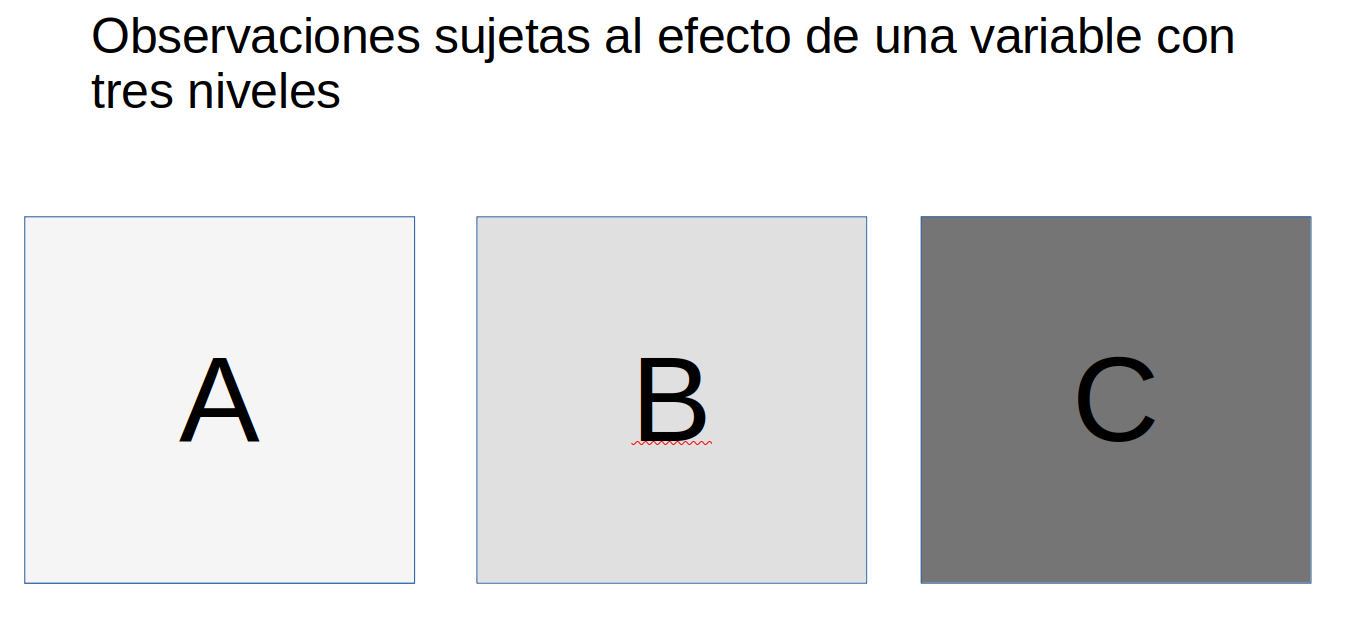
\includegraphics{Figuras-disenos/Factoriales.png}
\end{frame}

\begin{frame}{Ejemplo}
\protect\hypertarget{ejemplo-1}{}
Efecto del tipo de suelo sobre tiempo de germinación de semillas de
palma:

\begin{itemize}
\tightlist
\item
  Suelo A - promedio de germinación 2 semanas
\item
  Suelo B - promedio de germinación 2.2 semanas
\item
  Suelo C - promedio de germinación 1.78 semanas
\end{itemize}
\end{frame}

\begin{frame}{Cohorte}
\protect\hypertarget{cohorte}{}
Se sigue por un largo período de tiempo a lxs individuos participantes y
registran eventos clave, objeto de estudio
\end{frame}

\begin{frame}{Ejemplo}
\protect\hypertarget{ejemplo-2}{}
En el experimento de germinación, se puede registrar

\begin{enumerate}
\tightlist
\item
  Fecha de inicio de experimento
\item
  Fecha de germinación
\item
  Fecha en que ocurrió primera floración
\item
  Fecha en que se detectó crecimiento de frutos
\item
  Número de frutos producidos
\item
  Número de descendientes en primera floración
\end{enumerate}
\end{frame}

\hypertarget{loguxedstica-de-los-experimentos}{%
\section{Logística de los
experimentos}\label{loguxedstica-de-los-experimentos}}

\begin{frame}{Características de diseños experimentales}
\protect\hypertarget{caracteruxedsticas-de-diseuxf1os-experimentales}{}
Cómo se asignan las unidades experimentales a los tratamientos

\begin{enumerate}
\item
  Aleatorizados
\item
  Replicados
\end{enumerate}
\end{frame}

\begin{frame}{Aleatorizados}
\protect\hypertarget{aleatorizados}{}
\begin{itemize}
\item
  Muestras seleccionadas al asar
\item
  Unidades experimentales asignadas al asar
\item
  Ubicación de unidades es aleatoria
\end{itemize}
\end{frame}

\begin{frame}{Réplicas}
\protect\hypertarget{ruxe9plicas}{}
\begin{itemize}
\item
  Tratamientos experimentales
\item
  Unidades experimentales
\item
  Sitios de muestreo
\end{itemize}
\end{frame}

\begin{frame}{Objetivo del diseño}
\protect\hypertarget{objetivo-del-diseuxf1o}{}
\begin{itemize}
\item
  Repetitividad

  \begin{itemize}
  \item
    Que las hipótesis probadas sean predictivas a escalas comparables
  \item
    En otros experimentos
  \item
    En contextos más amplios que experimentales
  \end{itemize}
\end{itemize}
\end{frame}

\begin{frame}{Relación entre diseño e hipótesis}
\protect\hypertarget{relaciuxf3n-entre-diseuxf1o-e-hipuxf3tesis}{}
\begin{itemize}
\item
  Diseño debe permitir probar hipótesis estadística
\item
  Factorial

  \begin{itemize}
  \item
    Factor = variable independiente
  \item
    Variables medidas = variable dependiente
  \end{itemize}
\end{itemize}
\end{frame}

\begin{frame}{Tipos}
\protect\hypertarget{tipos}{}
\begin{enumerate}
\item
  Completamente aleatorizado
\item
  Bloques aleatorizados
\item
  Cuadrado latino
\item
  Split Plot, o parcelas divididas
\item
  Rejilla
\item
  Aumentados
\end{enumerate}
\end{frame}

\begin{frame}{Aleatorizado}
\protect\hypertarget{aleatorizado}{}
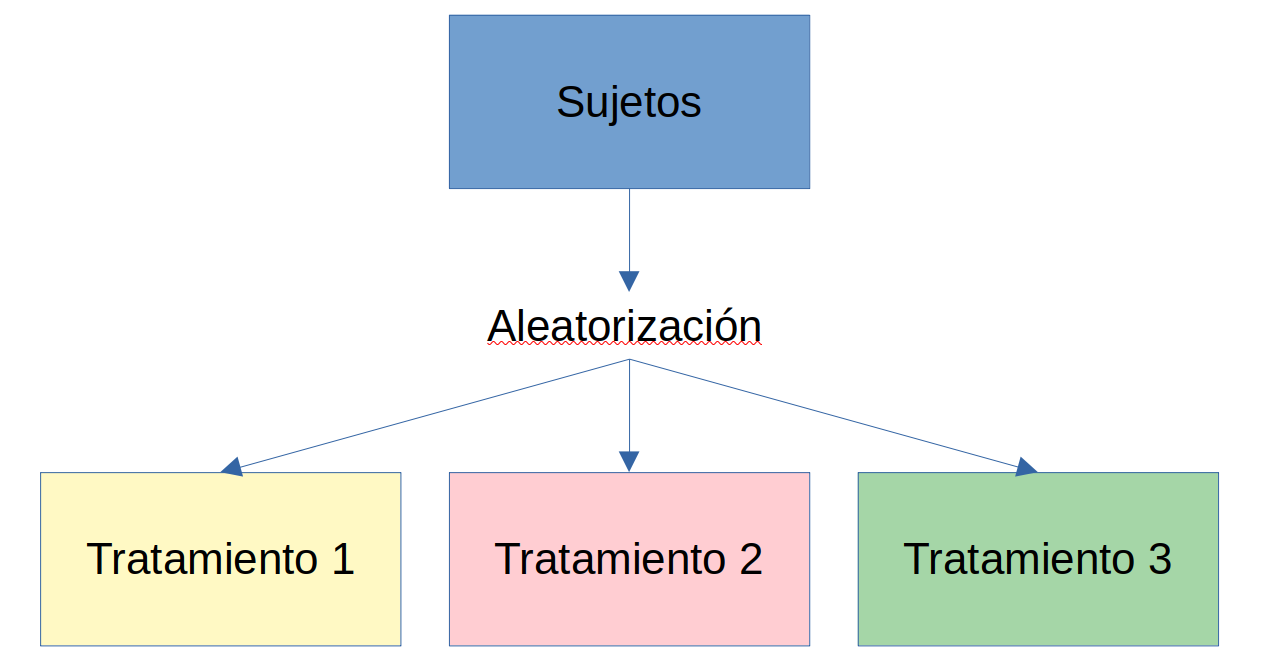
\includegraphics{Figuras-disenos/Aleatorizado.png}
\end{frame}

\begin{frame}{Bloques aleatorios}
\protect\hypertarget{bloques-aleatorios}{}
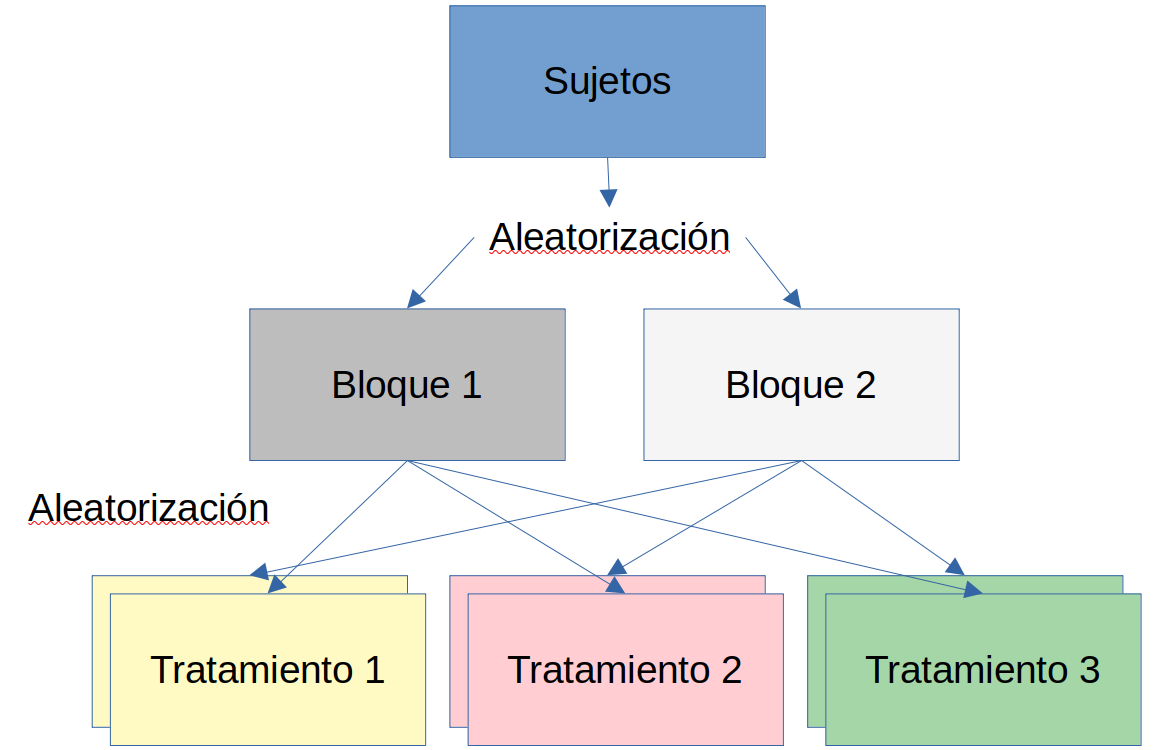
\includegraphics{Figuras-disenos/Bloques.png}
\end{frame}

\begin{frame}{Cuadrado latino}
\protect\hypertarget{cuadrado-latino}{}
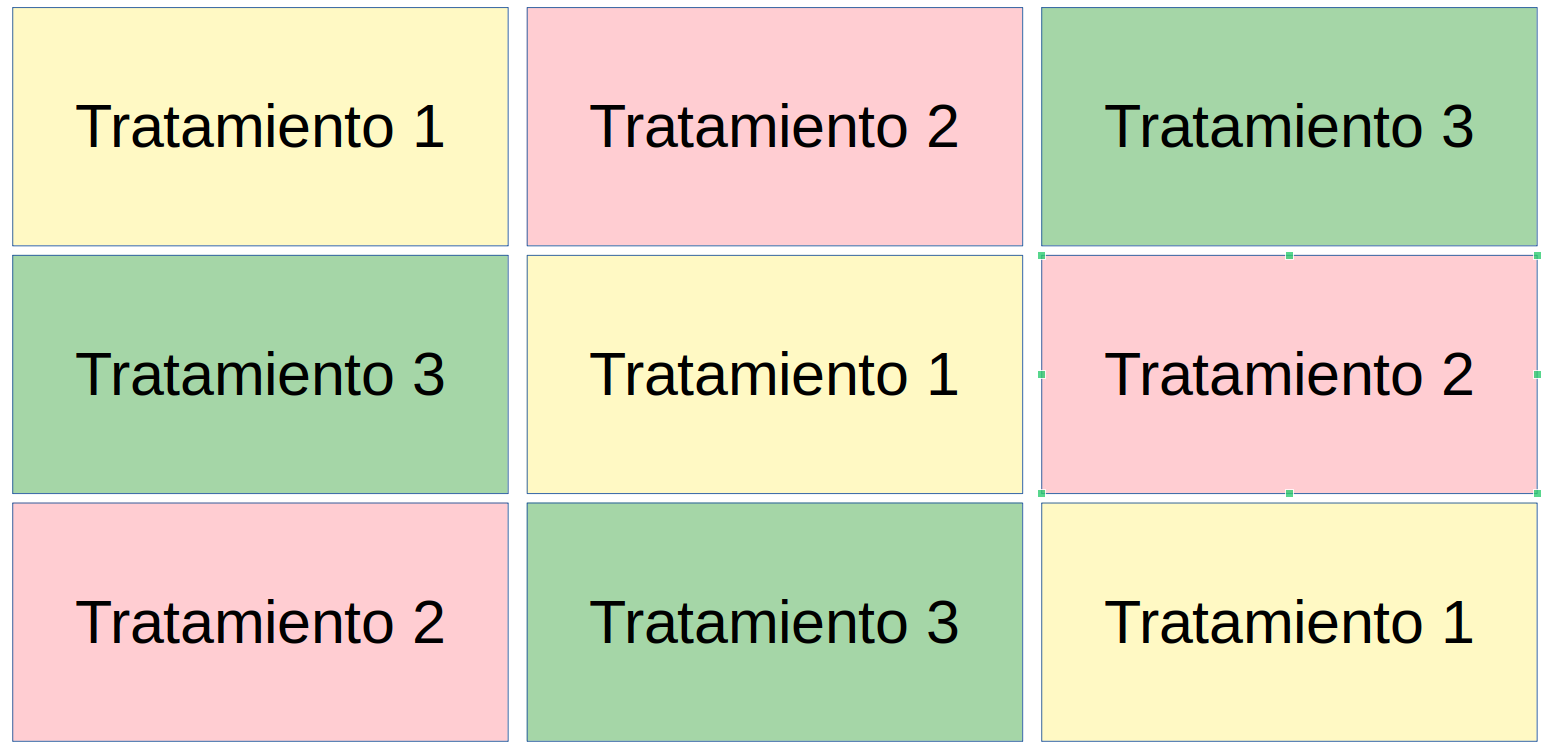
\includegraphics{Figuras-disenos/Cuadrado-latino.png}
\end{frame}

\begin{frame}{Split plot}
\protect\hypertarget{split-plot}{}
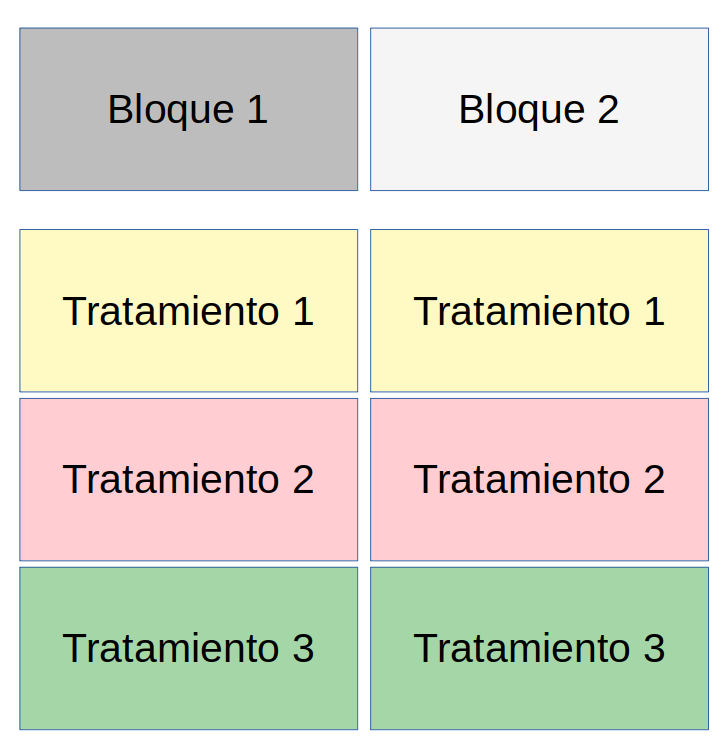
\includegraphics{Figuras-disenos/Split-plot.png}
\end{frame}

\begin{frame}{Rejilla}
\protect\hypertarget{rejilla}{}
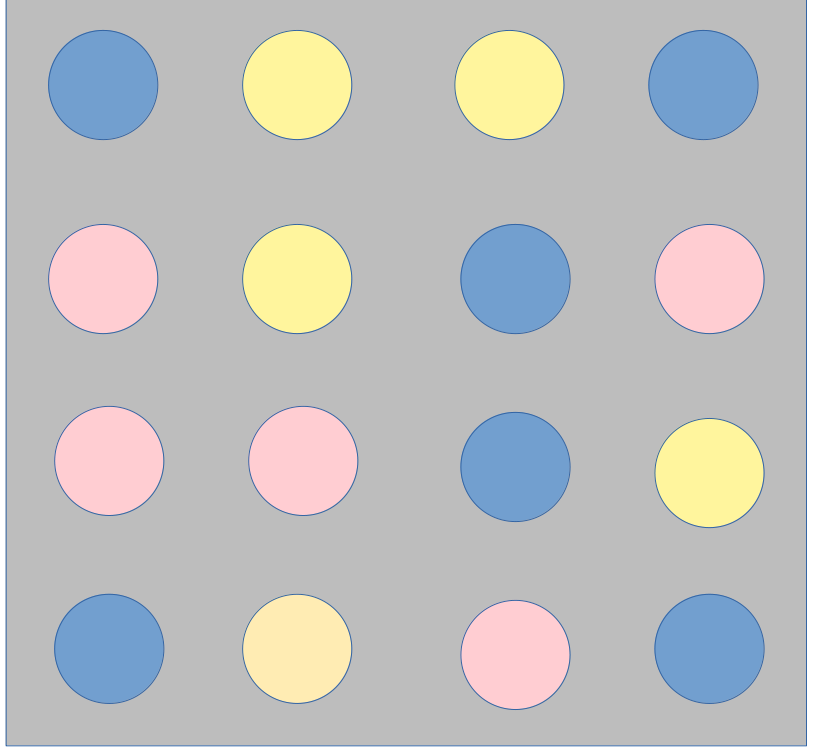
\includegraphics{Figuras-disenos/Rejilla.png}
\end{frame}

\hypertarget{relaciuxf3n-entre-diseuxf1o-y-anuxe1lisis}{%
\section{Relación entre diseño y
análisis}\label{relaciuxf3n-entre-diseuxf1o-y-anuxe1lisis}}

\begin{frame}[fragile]{Tipos de variables observacionales}
\protect\hypertarget{tipos-de-variables-observacionales}{}
Numéricas:

\begin{verbatim}
- Regresión lineal
- ANOVA
- Modelos lineales generalizados
\end{verbatim}
\end{frame}

\begin{frame}[fragile]{Variables contínuas}
\protect\hypertarget{variables-contuxednuas}{}
Positivas ó negativas

\begin{verbatim}
- Regresión lineal
- ANOVA
\end{verbatim}

Variables independientes contínuas y/o categóricas:

\begin{verbatim}
- Regresión lineal
\end{verbatim}

Variables independientes categóricas únicamente:

\begin{verbatim}
- Regreción lineal
- ANOVA
\end{verbatim}
\end{frame}

\begin{frame}[fragile]{Variables contínuas}
\protect\hypertarget{variables-contuxednuas-1}{}
Estrictamente positivas (p.~ej. precipitación, tiempo)

\begin{verbatim}
- Modelos lineales generalizados
    - log-normal
    - Gamma (más recomendado para tiempo)
    
\end{verbatim}
\end{frame}

\begin{frame}[fragile]{Variables discretas}
\protect\hypertarget{variables-discretas}{}
Variables discretas, sin decimales, p.~ej. conteos poblacionales

\begin{verbatim}
- Modelos lineales generalizados
    - Poisson
    - Logística, binomial (también para binarias, 1, 0)
    
\end{verbatim}
\end{frame}

\hypertarget{factores-de-agrupamiento}{%
\section{Factores de agrupamiento}\label{factores-de-agrupamiento}}

\begin{frame}{Bloques}
\protect\hypertarget{bloques}{}
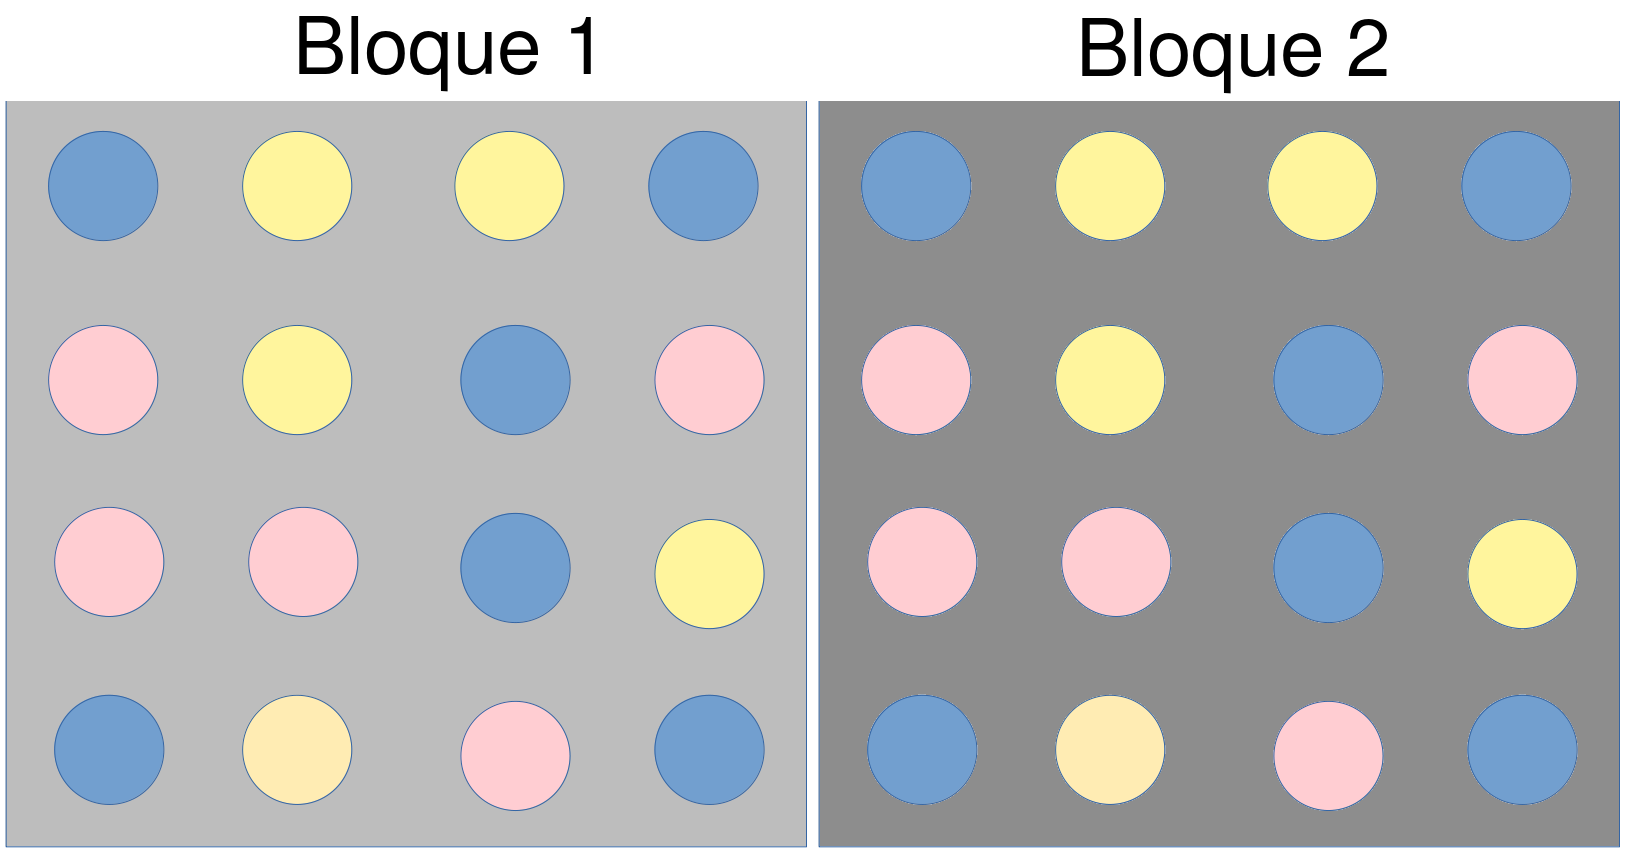
\includegraphics{Figuras-disenos/Rejilla-bloques.png}
\end{frame}

\begin{frame}{Bloques}
\protect\hypertarget{bloques-1}{}
\begin{itemize}
\item
  Tratamientos experimentales (Color de las bolitas)
\item
  Agrupamiento: bloques (Cajas de color gris)
\item
  Implicaciones para análisis:

  \begin{itemize}
  \item
    Tratamientos: efectos fijos - Factores cuyo efecto sobre objeto de
    estudio deseamos medir
  \item
    Bloques: efectos aleatorios - Factores no medidos, desconocidos que
    aumentan variabilidad
  \end{itemize}
\end{itemize}
\end{frame}

\begin{frame}{Ejemplo del efecto de los bloques}
\protect\hypertarget{ejemplo-del-efecto-de-los-bloques}{}
\begin{center}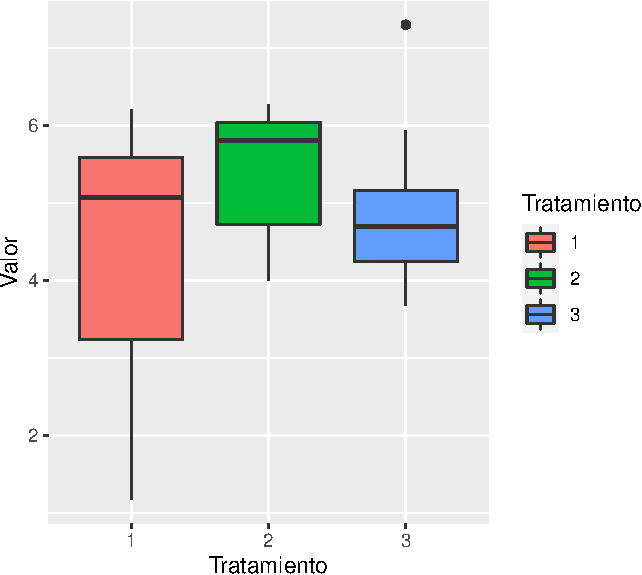
\includegraphics{Relacion-diseno-analisis_files/figure-beamer/unnamed-chunk-1-1} \end{center}
\end{frame}

\begin{frame}{Ejemplo del efecto de los bloques}
\protect\hypertarget{ejemplo-del-efecto-de-los-bloques-1}{}
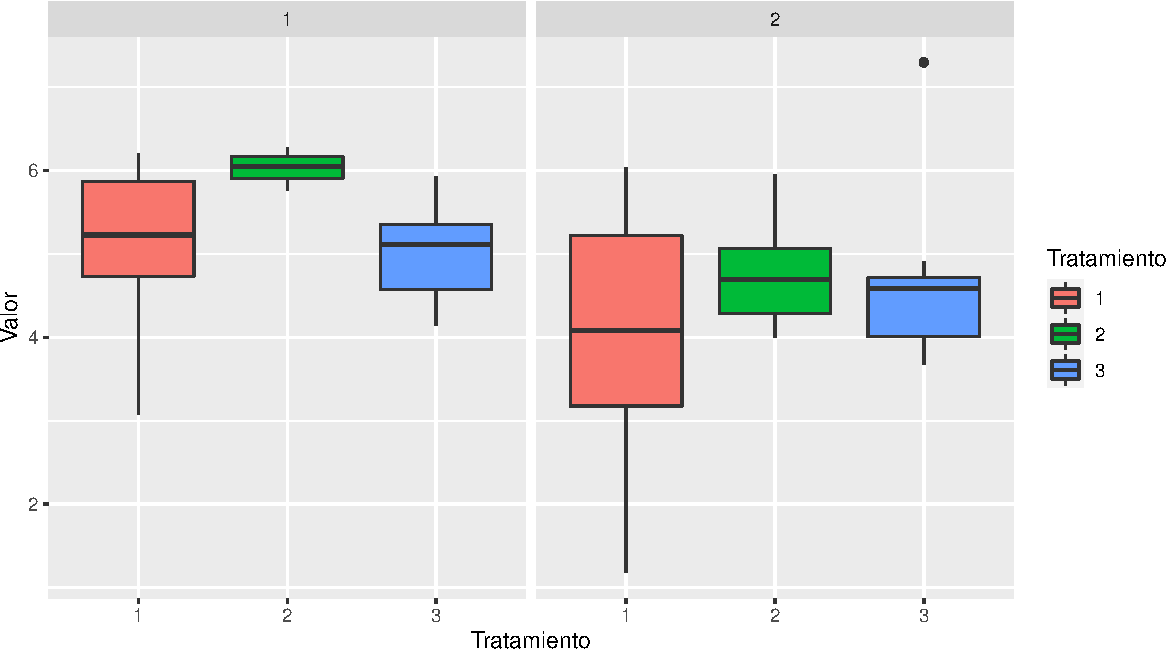
\includegraphics{Relacion-diseno-analisis_files/figure-beamer/unnamed-chunk-2-1.pdf}
\end{frame}

\begin{frame}{Efecto de bloques y tratamientos}
\protect\hypertarget{efecto-de-bloques-y-tratamientos}{}
\begin{itemize}
\item
  Bloques afectan dispersión (varianza)
\item
  Tratamientos afectan promedio
\end{itemize}
\end{frame}

\end{document}
